%PAGINA 1

\begin{frame}
\frametitle{Diseño e Implementación}
\framesubtitle{Electrónica Digital}
Componentes de electrónica digital utilizados:
\begin{itemize}
    \item Microcontrolador: Arduino Nano.
    \item Datalogger: Openlog Sparkfun.
    \item Sensor barométrico y de temperatura: MS5611.
    \item Sensor de corriente por efecto Hall: ACS723.
\end{itemize}
\end{frame}



%PAGINA 4
\begin{frame}
    \frametitle{Diseño e Implementación}
    \framesubtitle{Etapa de potencia para carga útil}
    \vfill
    \begin{figure}
        \centering
        \begin{minipage}{.5\textwidth}
            \centering
            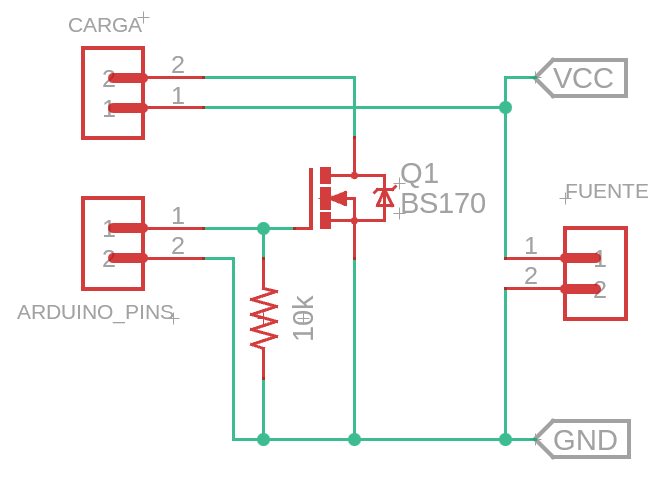
\includegraphics[width=0.6\textheight]{EtapaMosfet_Esquematico.png} % Reemplaza con tu primera imagen
            \mycaption{Esquemático de estapa con MOSFET BS170}
            \label{fig:ESQMOSFET}
        \end{minipage}\hfill
        \begin{minipage}{.5\textwidth}
            \centering
            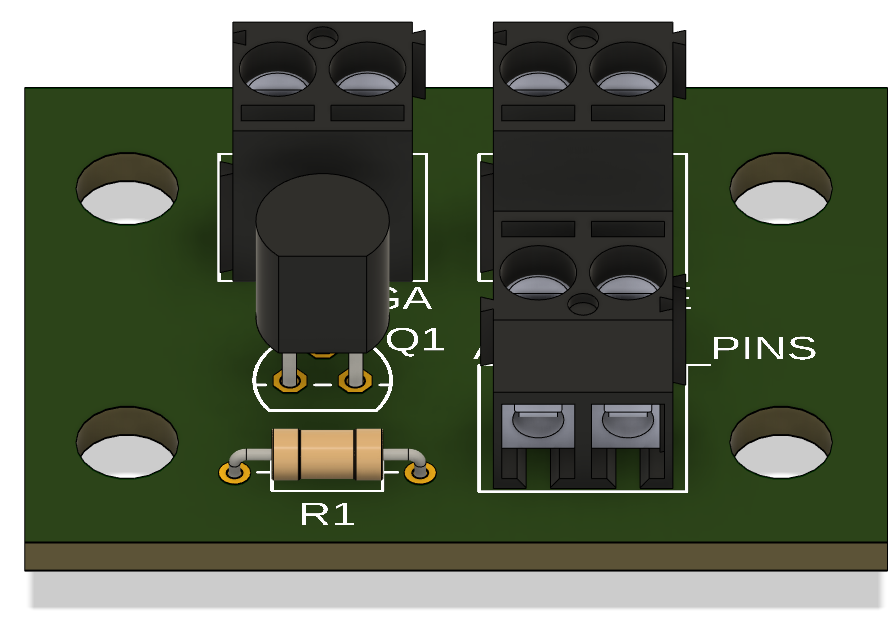
\includegraphics[width=.6\textheight]{3D_MOSFET.png} % Reemplaza con tu segunda imagen
            \mycaption{PCB de estapa con MOSFET BS170}
            \label{fig:PCBMOSFET}
        \end{minipage}
    \end{figure} 
\end{frame}


%PAGINA 6
\begin{frame}
    \frametitle{Diseño e Implementación}
    \framesubtitle{Baterías}
    \begin{figure}[H]
        \centering
        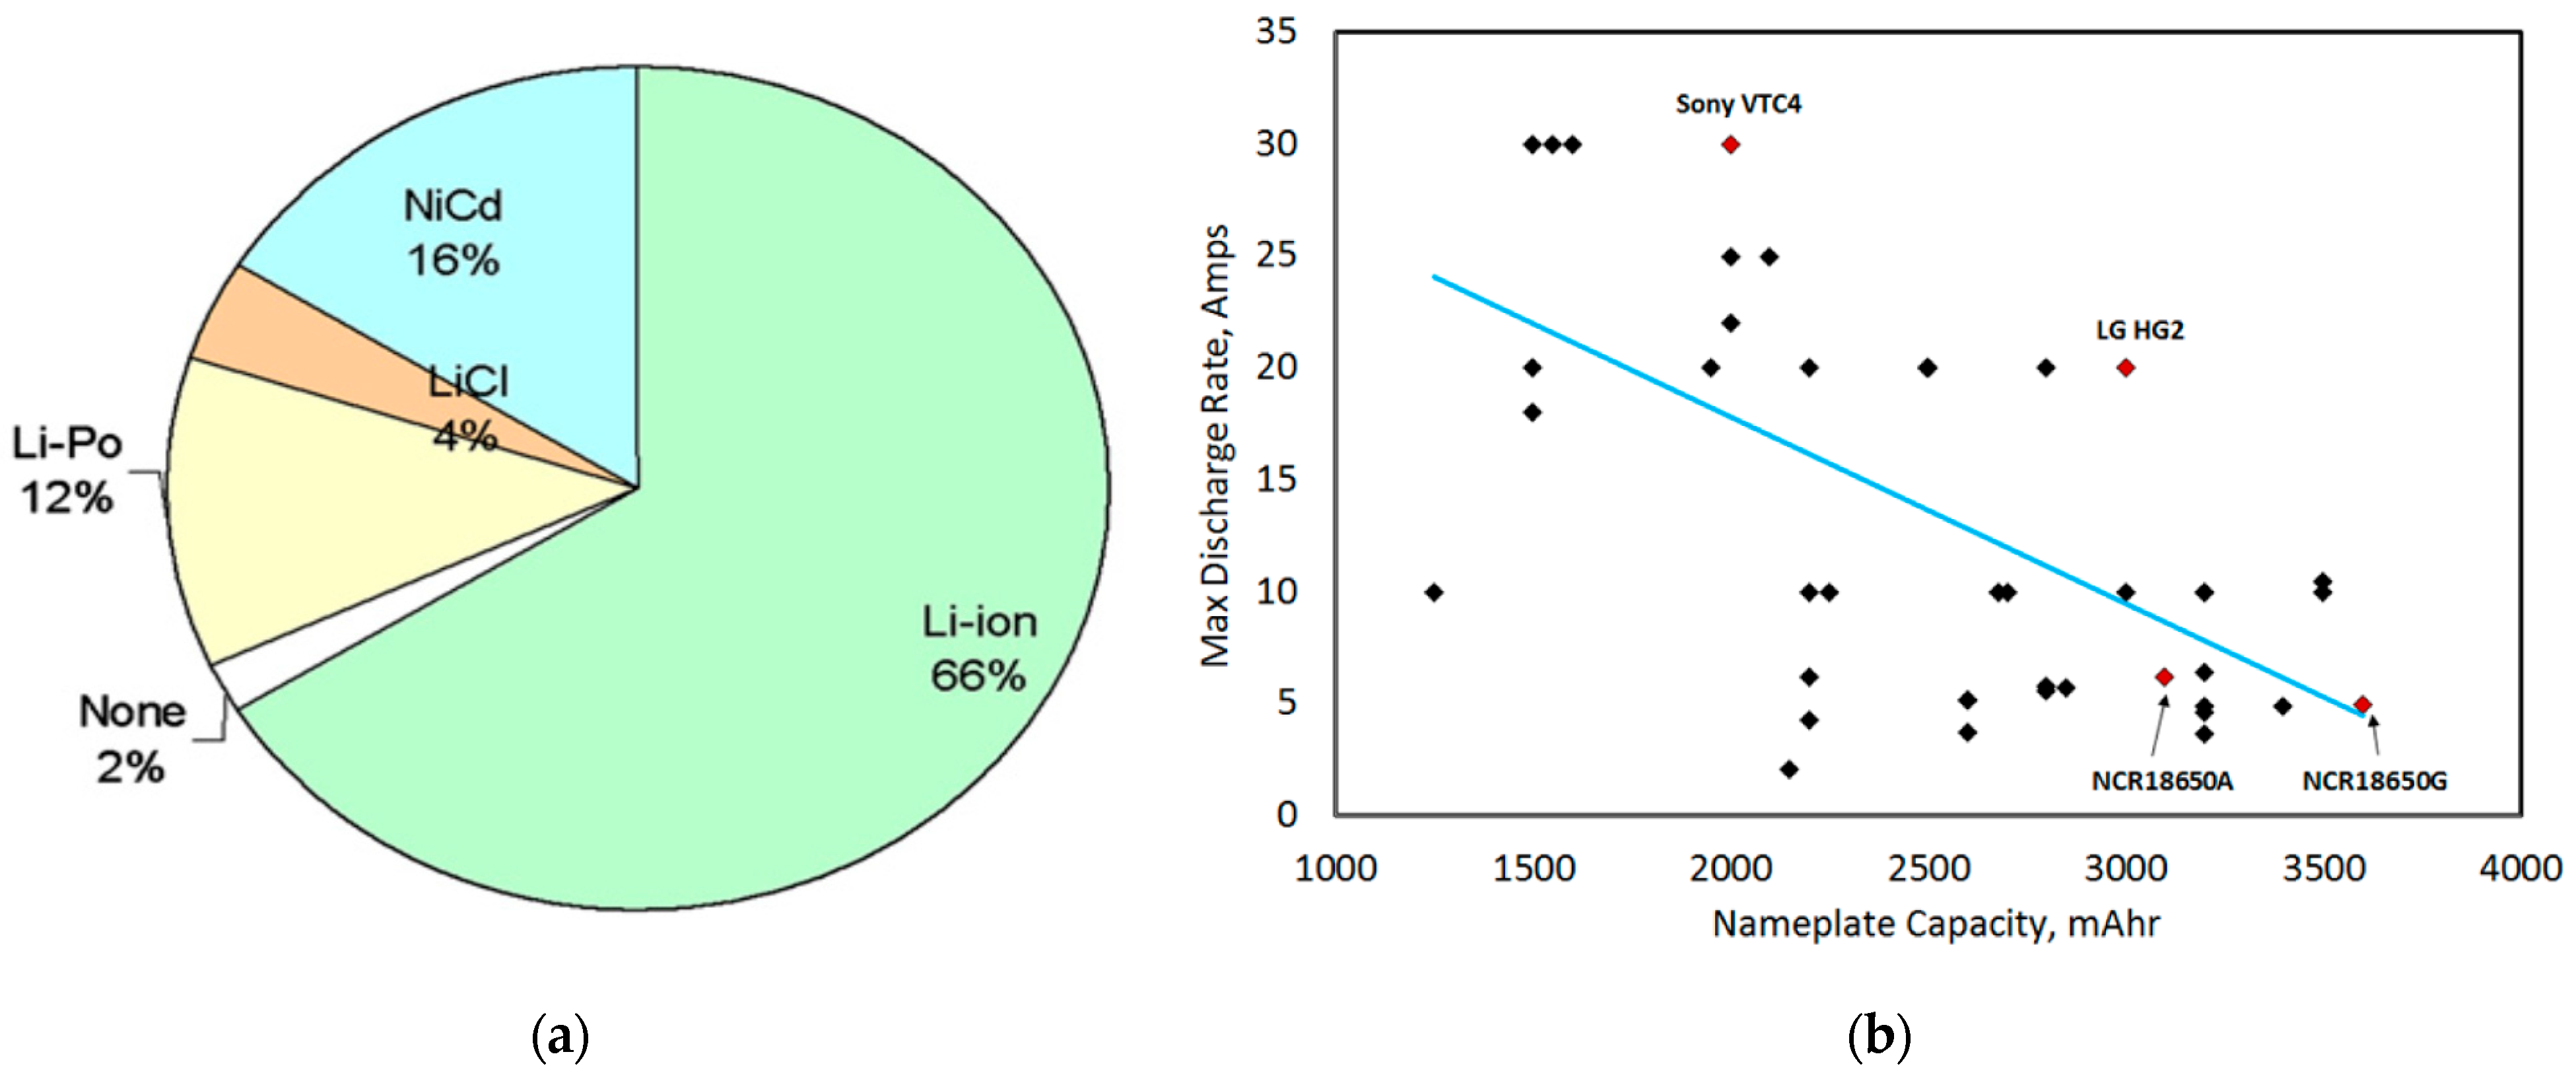
\includegraphics[width=0.8\textwidth]{COTSBatteries.png} % Ajusta el tamaño según sea necesario
        \mycaption{(a) Battery types used in pico- and nano-satellites[41]. (b) Summary of
        maximum discharge rate capabilities versus nameplate capacity of some representative
        COTS 18650 Li-ion cells \cite{chin2018energy}}
        \label{fig:COTSBatt}
    \end{figure}
    

\end{frame}


%PAGINA 7
\begin{frame}
    \frametitle{Diseño e Implementación}
    \framesubtitle{Baterías}
    Se seleccionó el modelo Panasonic NCR18650B por su corriente máxima de descarga de 4.9 A y capacidad nominal de 3400 mAh. Basándose en el presupuesto energético, se optó por un arreglo de 4 baterías. Para examinar la operatividad de etapas subsiguientes, como los convertidores DC-DC, se consideraron tres configuraciones: 
    \begin{itemize}
        \item 4s1p
        \item 2s2p
        \item 1s4p
    \end{itemize}
\end{frame}

%PAGINA 8
\begin{frame}
    \frametitle{Diseño e Implementación}
    \framesubtitle{Convertidores DC-DC}
    Aunque los convertidores lineales son baratos y simples, su eficiencia limitada, dada por $E = \frac{V_{\text{out}}}{V_{\text{in}}} \times 100\%$, conduce a una caída notable de eficiencia, como se ilustra en la Fig.\ref{fig:LDOE}.
    \begin{figure}[H]
        \centering
        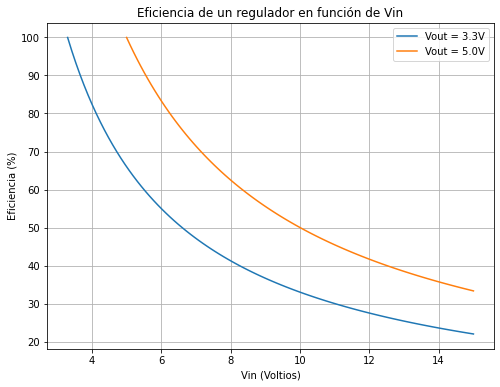
\includegraphics[width=0.5\textwidth]{Grafica_Eficiencia_LDO.png} % Ajusta el tamaño según sea necesario
        \mycaption{Eficiencia del regulador LT1117 en función del Vin}
        \label{fig:LDOE}
    \end{figure}
\end{frame}




%PAGINA 11

\begin{frame}
    \frametitle{Diseño e Implementación}
    \framesubtitle{Convertidores DC-DC: Arreglo 4s1p}
    \begin{figure}[H]
        \centering
        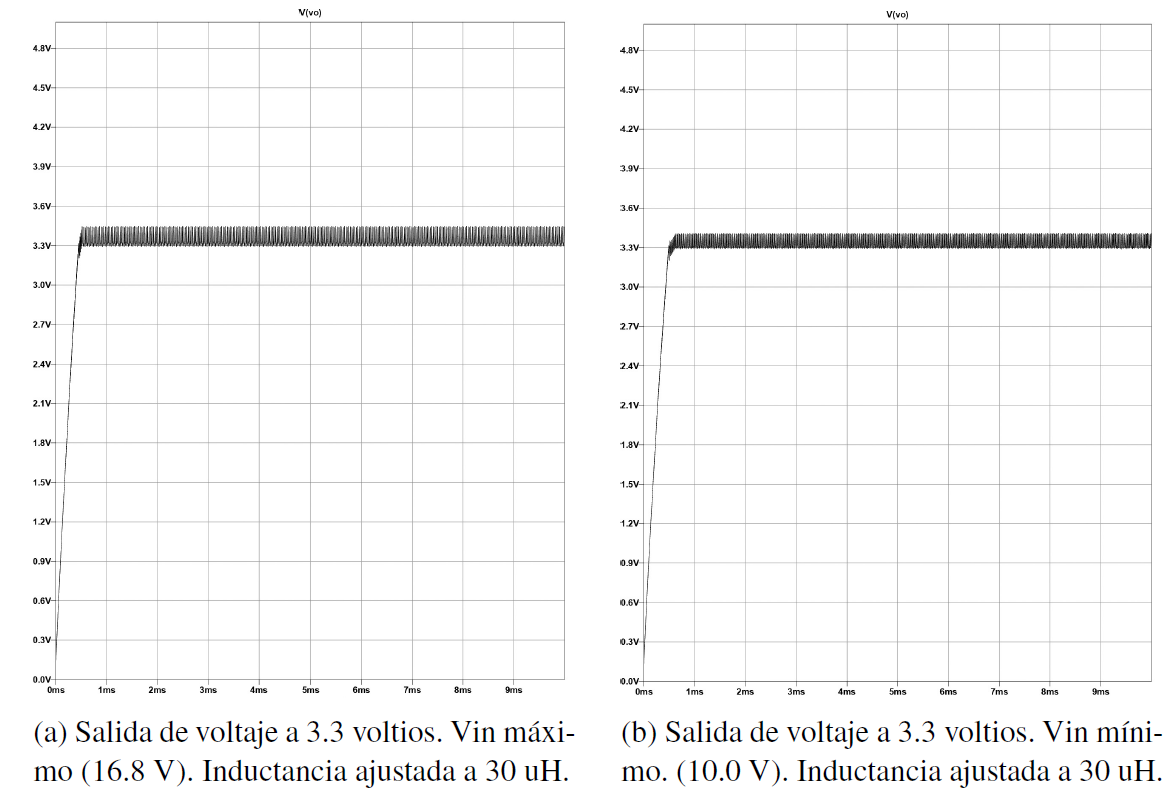
\includegraphics[width=0.7\textwidth]{4S1P_A.png} % Ajusta el tamaño según sea necesario
        \mycaption{Convertidor DC-DC MC34063A, arreglo 4s1p, bus de 3.3 V a 750 mA.}
        \label{fig:4S1P_A}
    \end{figure}
\end{frame}

%PAGINA 16

\begin{figure}
    \frametitle{Diseño e Implementación}
    \framesubtitle{Convertidores DC-DC: Esquemático Bus 3.3 V}
    \begin{figure}[H]
        \centering
        \includegraphics[width=0.9\textwidth]{MC34063A_Esquemático_33V.png} % Ajusta el tamaño según sea necesario
        \mycaption{Convertidor DC-DC MC34063A, arreglo 4s1p, bus de 3.3 V a 750 mA.}
        \label{fig:Resultado3.3}
    \end{figure}
\end{figure}


%PAGINA 12
\begin{frame}
    \frametitle{Diseño e Implementación}
    \framesubtitle{Convertidores DC-DC: Arreglo 4s1p}
    \begin{figure}[H]
        \centering
        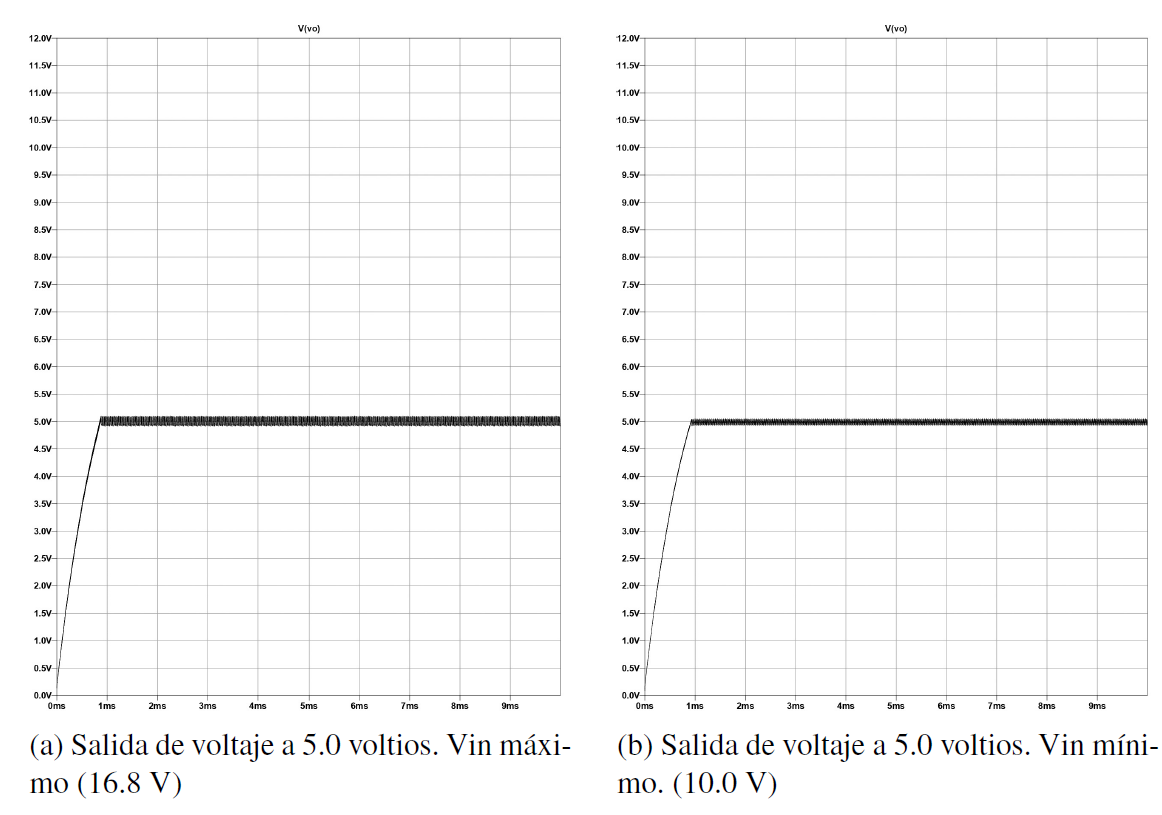
\includegraphics[width=0.7\textwidth]{4S1P_B.png} % Ajusta el tamaño según sea necesario
        \mycaption{Convertidor DC-DC MC34063A, arreglo 4s1p, bus de 5.0 V a 750 mA.}
        \label{fig:4S1P_B}
    \end{figure}
\end{frame}




%PAGINA 17

\begin{figure}
    \frametitle{Diseño e Implementación}
    \framesubtitle{Convertidores DC-DC: Esquemático Bus 5.0 V}
    \begin{figure}[H]
        \centering
        \includegraphics[width=0.9\textwidth]{MC34063A_Esquemático_50V.png} % Ajusta el tamaño según sea necesario
        \mycaption{Convertidor DC-DC MC34063A, arreglo 4s1p, bus de 5.0 V a 750 mA.}
        \label{fig:Resultado5.0}
    \end{figure}
\end{figure}


%PAGINA 17
\begin{frame}
\frametitle{Diseño e Implementación}
\framesubtitle{Circuito de Protección: Limitador de corriente}
\begin{figure}
    \begin{figure}[b]
        \centering
        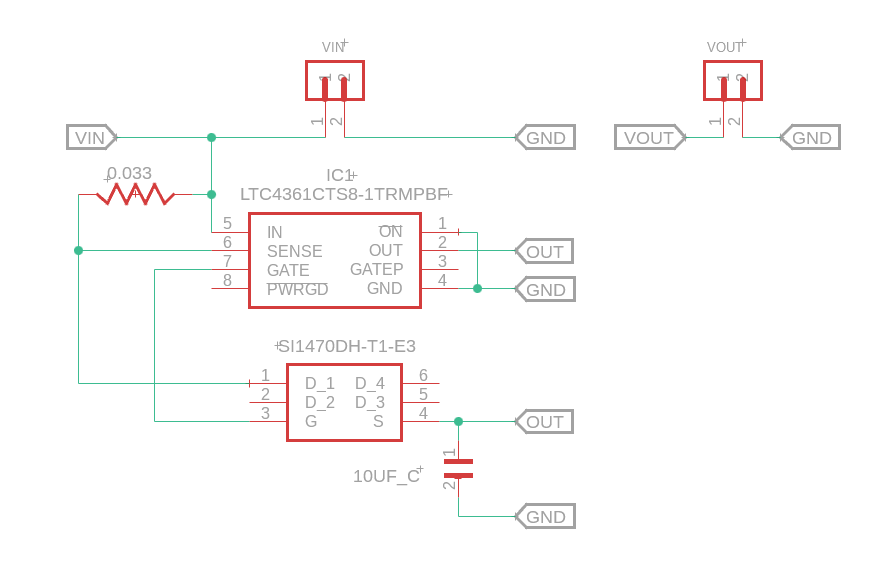
\includegraphics[width=0.75\textwidth]{Esquematico_LTC4361.png} % Ajusta el tamaño según sea necesario     
        \mycaption{Circuito de protección LTC4361. \( R_{\text{sense}} = 0.033\,\Omega \) para \( I_{\text{trip}} = 1.5\,A \). PCB de material FR-4 (0.762\,mm), \( I_{\text{máx}} = 2\,A \) \cite{LTC4361}\cite{altiumfr4}.}
        \label{fig:Resultado6.0}
    \end{figure}
\end{figure}
\end{frame}